% !TEX root = ../termpaper.tex
% @author Kjell May
%
\graphicspath{{chapters/images/}}
\section{Einleitung}
Minesweeper ist ein klassisches Rätsel-/ Puzzlespiel von Microsoft Windows, welches auf früheren Windows-Versionen
vorinstalliert gewesen ist. In dem Spiel geht es darum, alle Felder auf einem Spielfeld aufzudecken, unter denen
sich keine Mine befindet. Schafft man das, hat man gewonnen, ansonsten verliert man das Spiel. Um dieses Ziel zu
erreichen und die Minen zu lokalisieren, gibt das Spiel einem Hinweise in Form von Zahlen auf aufgedeckten
Feldern, welche die Anzahl der umgebenden Minen beschreiben. Ein Beispiel eines gelösten Spiels könnte so aussehen (entnommen von \cite{MS}):

\begin{figure}[!htb]
    \captionsetup{font=small,labelfont={bf,sf}}
    \centering
    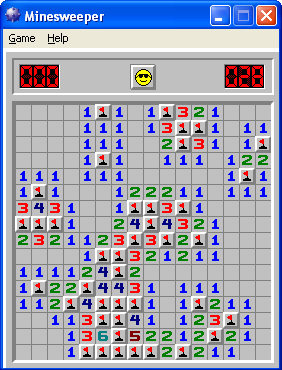
\includegraphics[scale=0.7]{finished}
    \caption{Ein beendetes Spiel auf Windows XP}\label{finished}
\end{figure}